\documentclass[../sparc.tex]{subfiles}
\graphicspath{{\subfix{../images/}}}
\begin{document}

%%%%%%%%%%%%%%%%%%%%%%%%%%%%%%%%%%%%%%%%%%%%%%%%%%%%%%%%%%%%%%%%%%%%%%%%%%%%%%%%
\section{Serial port}
\label{section:communication-serial-port}
\index{Electronics!Serial port}

%%%%%%%%%%%%%%%%%%%%%%%%%%%%%%%%%%%%%%%%%%%%%%%%%%%%%%%%%%%%%%%%%%%%%%%%%%%%%%%%
\subsection{General information}

\emph{Serial port} is one of the simplest ways of communication between digital
devices.  As it follows from its name the protocol transfers bits sequentially,
one bit at the time.  There are other hardware interfaces that also use serial
data transfer -- for example, USB and Ethernet.  But under the term ``serial
port'' most people mean the hardware that is compatible with the RS-232 and
other related standards (e.g. RS-485, RS-422 and others.)

A serial port usually implements the \emph{full-duplex} communication as it
allows to transfer data in both directions simultaneously.  For that two
independent lines are used: one for transferring the data (``Transmit'' or
``Tx'') and another for receiving the data (``Receive'' or ``Rx''.)

We may wonder why usually ``Receive'' is shortened to ``Rx'' and ``Transmit'' to
``Tx''. The reason for that can be found in the history: back in the times when
telegraph was in use it was easier to send a letter than to send a dot, thus
operators used ``x'' letter in the place of a dot.

The cost of telegraph usage was fixed and it included the salary of an operator,
the cost of printer usage and the cost of the telegraph line between the
stations.  The more data you could transfer, the more money you could earn.
That lead to the shear number of shorthands for the common words, especially
long ones.  Thus instead of the long word ``Transmission'' telegraph operators
preferred to use just ``T.'' (knowing that on the receiving site they will be
understood.)  But the dot symbol wasn't available in telegraph when the letter
input mode was active.  That forced operators to input ``T'' letter, then switch
telegraph to the numbers input mode (to input a dot symbol) and then switch back
to the letter input mode.  That took a long time.  Thus each time when it was
needed to send a dot, telegraphers used ``X'' symbol instead, that could be
written without switching to the number input mode.  Because very small number
of English words end with ``X'' this symbol turned out to be an ideal
replacement for a dot.

That the origin of such shorthands as ``Rx'' and ``Tx''.\autocite{so:krisw}

One drawback of the serial port is a lower data transfer speed comparing to the
\emph{parallel port}, where you can transfer eight bit simultaneously.  But to
transfer 8 bits once over the parallel port we have to have 8 wires connecting
the transmitter and the receiver, while the serial port only requires one wire
for data transfer.  Thus the serial data transfer bus is more compact.

%%%%%%%%%%%%%%%%%%%%%%%%%%%%%%%%%%%%%%%%%%%%%%%%%%%%%%%%%%%%%%%%%%%%%%%%%%%%%%%%
\subsection{Universal Asynchronous Receiver-Transmitter (UART)}
\label{section:communication-uart}

The universal asynchronous receiver-transmitter, widely known as \emph{UART} --
is a special device or a logical circuit for asynchronous serial data transfer.
In fact UART is one of the implementations of the serial port that is commonly
used for data exchange between devices.

On the transmitting side, UART receives data and sequentially transmits them as
separate bits over the bus, one after another, with equal periods of time.  On
the receiver the second UART assembles received bits into the original bytes.
Both the transmitter and the receiver have a special chip called \emph{shift
register} which provides a fundamental way to convert the data between the
serial and the parallel representation.

%% TODO: Insert an image of a shift register (parallel-to-serial and
%% serial-to-parallel.)

An example of 1 byte of information transfer is visualized as a diagram on fig.
\ref{fig:communication-serial-port-diagram}.  The diagram shows the change of
voltage in time on the line Rx-Tx between two devices.

\figureSerialPortDiagram{en}

The speed of data transfer is determined by the parameter called \emph{bit rate}
or \emph{baud rate}, which is measured in bauds (bits per second.)  The speed
$S$ (in bauds) and the length of one bit $T$ (in seconds) are linked together by
the relation \ref{equation:uart-speed}.

\begin{equation}
  T = \frac{1}{S}
  \label{equation:uart-speed}
\end{equation}

Where $T$ is the length of one bit and it depends on the speed of data transfer
(see the fig. \ref{fig:communication-serial-port-diagram}.)

Common baud rates are: 300, 1200, 2400, 4800, 9600, 19200, 38400, 57600, 115200,
230400, 460800 and 921600 baud.

If we substitute 9600 baud in the equation \ref{equation:uart-speed} we get:

\begin{equation}
  T = \frac{1}{9600} \approx 0.00010416 \mbox{s} \approx 104.16 \mu\mbox{s}
\end{equation}

Thus for the 9600 baud the time to transfer one bit is roughly $104.16
\mu\mbox{s}$.  For comparison, the minimal blink time for human eyes is $\approx100
\mbox{us}$\cite{chudler}, which is $\approx960$ times slower than the one bit
transferring time with that speed.

It should be noted that for successful communication both transmitter and
receiver must have the same serial port speed, otherwise data will not be read
correctly.  This is due to the fact that the transmitter and the receiver don't
have the clock signal that synchronizes data transfer.

Sometimes it is more convenient to operate not with bits per second, but rather
with bytes with seconds, as in common situations we specifically measure the
amount of information in bytes.  In the most cases one byte contains 8 bits.

At the first glance it is logical to conclude that we can get the number of
bytes per second by using the equation
\ref{equation:uart-bauds-to-bytes-per-sec-1}.

\begin{equation}
  S_{\mbox{bytes/s}} = \frac{S_{\mbox{bits/s}}}{8}
  \label{equation:uart-bauds-to-bytes-per-sec-1}
\end{equation}

But we have to take into account that each byte sent is preceded by the start
bit and followed by the end bit.  Thus the actual speed of data transfer is
lower (see the equation \ref{equation:uart-bauds-to-bytes-per-sec-2}.)

\begin{equation}
  S_{\mbox{bytes/s}} = \frac{S_{\mbox{bits/s}}}{8 + 1 \mbox{start bit} + 1 \mbox{stop bit}}
  \label{equation:uart-bauds-to-bytes-per-sec-2}
\end{equation}

\example { One of the popular data transferring speeds is 9600 bauds.  Using the
  equation \ref{equation:uart-bauds-to-bytes-per-sec-2} we can calculate how
  many bytes we can transfer in one second between a computer and an Arduino:

  \begin{equation}
    S_{\mbox{bytes/s}} = \frac{9600_{\mbox{bits/s}}}{10} = 960 \mbox{bytes/s} \approx 0.93 \mbox{KB/s}
  \end{equation}

  Let's assume that one musical composition is 5MB in size on average.  If we
  would want to transfer this file from the computer to the Arduino with 9600
  baud speed, we can calculate how much time would be required for that:

  \begin{align*}
    5 MB = 5242880 bytes\\
    T = \frac{5242880 bytes}{960 bytes} \approx 5461.33 s \approx 91 minutes
  \end{align*}

  Thus we calculated that for transferring of 5MB of data we need at least 91
  minutes -- that is, around 1.5 hours.
}

%%%%%%%%%%%%%%%%%%%%%%%%%%%%%%%%%%%%%%%%%%%%%%%%%%%%%%%%%%%%%%%%%%%%%%%%%%%%%%%%
\subsection{Working with a serial port}

\subsubsection{\texttt{Serial} class}

In Arduino, there is a class for working with a serial port named
\texttt{Serial}, that allows us to configure \gls{UART} parameters, to transmit
and to receive the data.  We already worked with the serial port in the section
\ref{section:serial-port}, and now we discuss it in more depth.

On all Arduino boards there at least one serial port, and some boards we have
more than one.  A list of serial ports and digital ports associated with them
can be found in the table \ref{table:serial-ports--pins} (the data is taken from
the description of \texttt{Serial} class from the \cite{arduino:reference}.)

\tableCommunicationSerialPorts{en}

On most of Arduino boards digital ports 0 (RX) and 1 (TX) is used by default for
the serial port.  Specifically this serial port (\texttt{Serial}) is used for
data transferring between a computer and an Arduino; thus the transferred data
is duplicated on the digital ports connected to this serial port.

%% TODO: Add a schematic of Arduino board with an USB-UART converter.

\note{en}{It must be noted that if we use the digital ports associated with the
  main \texttt{Serial} (usually those are digital ports 0 and 1), for example,
  for blinking LEDs -- it can interfere the correct uploading of a program to an
  Arduino.  In this case we may need to disconnect the external devices from
  ports 0 and 1 before uploading a new program.  That's why it is better not to
  use those ports without a good reason.}

%%%%%%%%%%%%%%%%%%%%%%%%%%%%%%%%%%%%%%%%%%%%%%%%%%%%%%%%%%%%%%%%%%%%%%%%%%%%%%%%
\subsubsection{Data transferring}

To transfer data to a computer, we need to configure the speed of data transfer.
It is reasonable to to this in \texttt{setup} procedure, as the speed is usually
set once and does not changes throughout the period of serial port use.

The setting of serial port speed is done using the \texttt{begin} method from
the \texttt{Serial} class.  In the following example we're setting the speed
equal to 9600 baud:

\begin{minted}{cpp}
  void setup() {
    Serial.begin(9600);
  }
\end{minted}

Next we can transfer some data to a computer.  For that there are methods
\texttt{print} and \texttt{println} in \texttt{Serial} class.  The main
difference between \texttt{println} and \texttt{print} methods is that
\texttt{println} sends a newline symbol at the end of data.

%% TODO: Add "write" description; add the description of data format for
%% "print"/"println".

An example of data transferring to a computer:

\begin{minted}{cpp}
  void loop() {
    Serial.println("Hello World");
  }
\end{minted}

It should be noted that the methods for data transferring allow us to work with
data of different types.  Thus, for example, we can transfer not only strings,
but also numbers using \texttt{println} -- a computer will ``figure out'' the
right way of preparing the data for the transfer:

\begin{minted}{cpp}
  void loop() {
    Serial.println(42);
  }
\end{minted}

All the data is converted into a string before the transfer, which then is sent
though the serial port.

%%%%%%%%%%%%%%%%%%%%%%%%%%%%%%%%%%%%%%%%%%%%%%%%%%%%%%%%%%%%%%%%%%%%%%%%%%%%%%%%
\subsection{Receiving the data}

\texttt{Serial} class provides a set of methods for reading data from the serial
port.

The data which is coming from a computer is buffered on the Arduino side.  The
size of the buffer is 64 bytes (see the documentation for the method
\texttt{available} of \texttt{Serial} class in \cite{arduino:reference}.)  Among
other methods \texttt{Serial} provides \texttt{available} method that returns
the number of bytes in the buffer that are available for reading.  Usually this
method is used right before the data reading.

The reading can be done using several methods, depending on the data type.  The
most primitive way is to read bytes with the \texttt{read} method.  Each call to
\texttt{read} returns the next available byte from the input buffer.  When there
is no data in the buffer, \texttt{read} returns -1 as the value.

\note{en}{ It should be noted that \texttt{read} returns \texttt{int} type
  instead of \texttt{byte} or \texttt{char}.  That is due to the fact that if
  \texttt{read} would return \texttt{byte} (which does not have the negative
  part), then it wouldn't be able to return -1, and without it we would not have
  a way to signal the end of data with the returned value.  On the other hand,
  if \texttt{read} would return \texttt{char}, this problem would be solved (as
  \texttt{char} has the range from -128 to 127), but at the same time we would
  have problems with receiving values from 128 to 255 (the maximal value, that
  can be written in one byte.) }

An example of data reading can be found in the listing below:

\begin{minted}{cpp}
  void loop() {
    if (Serial.available() > 0) {
      int incoming_byte = Serial.read();
      // ... Handling the data ...
    }
  }
\end{minted}

%%%%%%%%%%%%%%%%%%%%%%%%%%%%%%%%%%%%%%%%%%%%%%%%%%%%%%%%%%%%%%%%%%%%%%%%%%%%%%%%
\subsection{Software implementation of a serial port}

An embedded library
\texttt{SoftwareSerial}\footnote{\url{https://docs.arduino.cc/learn/built-in-libraries/software-serial/}}
bundled with Arduino IDE allows us to implement a serial port in software, using
custom digital ports that are different from the ones listed in the table
\ref{table:serial-ports--pins}.

With this library, we can implement several serial ports with speeds up to
115200 baud.

Nevertheless, \texttt{SoftwareSerial} has a bunch of serious drawbacks:
\begin{itemize}
\item The library allows us only to transfer or to receive data in each moment --
  that is, simultaneous transmitting and receiving is not possible. Thus we can
  say that such communication is performed in the \emph{half-duplex mode}.
\item If several \texttt{SoftwareSerial} are used then only one can receive data
  in each moment. This is due to the fact that data receiving is implemented
  through interrupts.
\item For receiving the data we have to use only those ports that support
  interrupts.
\item On Arduino and Genuino 101 boards the maximum data transfer speed is
  limited to 57600 baud.
\item On Arduino and Genuino 101 boards the 13th pin cannot be used as the RX
  port.
\end{itemize}

An example of software serial port usage is shown below.

\begin{listing}[H]
  \begin{minted}{cpp}
    #include <SoftwareSerial.h>

    const byte RX_PIN = 2;
    const byte TX_PIN = 3;

    SoftwareSerial my_serial(RX_PIN, TX_PIN);

    void setup() {
      my_serial.begin(9600);
      my_serial.println("Hello, World!");
    }

    void loop() {

    }
  \end{minted}
  \label{listing:communication-serial-software}
  \caption{An example of software serial port usage (\texttt{SoftwareSerial}.)}
\end{listing}

As this implementation of the serial port is based on the interrupt mechanism,
with high receiving speeds we can observe an effect called ``interrupt
starvation'' -- which means that an micro-controller spends most of its CPU time
handling interrupts and processing the incoming data, giving a minimal amount of
time to the rest of the tasks.  In t his case, for example, the \texttt{loop}
procedure will practically never be called, and the other interrupts (like ones
from external buttons) won't be processed as well.

%%%%%%%%%%%%%%%%%%%%%%%%%%%%%%%%%%%%%%%%%%%%%%%%%%%%%%%%%%%%%%%%%%%%%%%%%%%%%%%%
\subsection{Example: Transferring data between two Arduino boards}

Now we discuss a more complex example where we will see not only the usage of
the hardware serial port, but the software serial port as well.  For this we
need two Arduino boards between which we will transfer the data.

For data transferring we will use \texttt{SoftwareSerial} with digital ports
number 10 (RX) and 11 (TX.)  The first Arduino will transfer symbols
\texttt{'1'} and \texttt{'0'} alternately through the serial port to the second
Arduino.  In turn, the second Arduino will turn on an LED on receiving
\texttt{'1'} and turn it off on receiving \texttt{'0'}.

We must connect the digital port number 11 (TX) on the Arduino-transmitter to
the port number 10 (RX) on the Arduino-receiver.  Also we must connect ground
pins (\texttt{GND}) on both Arduino boards to ensure that they have the same
logical level for zero.  On fig. \ref{fig:arduino-serial-communication-1} we can
see an example of how to connect two Arduino Mega 2560 boards for this project.
We also can use other Arduino boards, given that we made required modifications
to the code.

\begin{figure}[H]
  \centering
  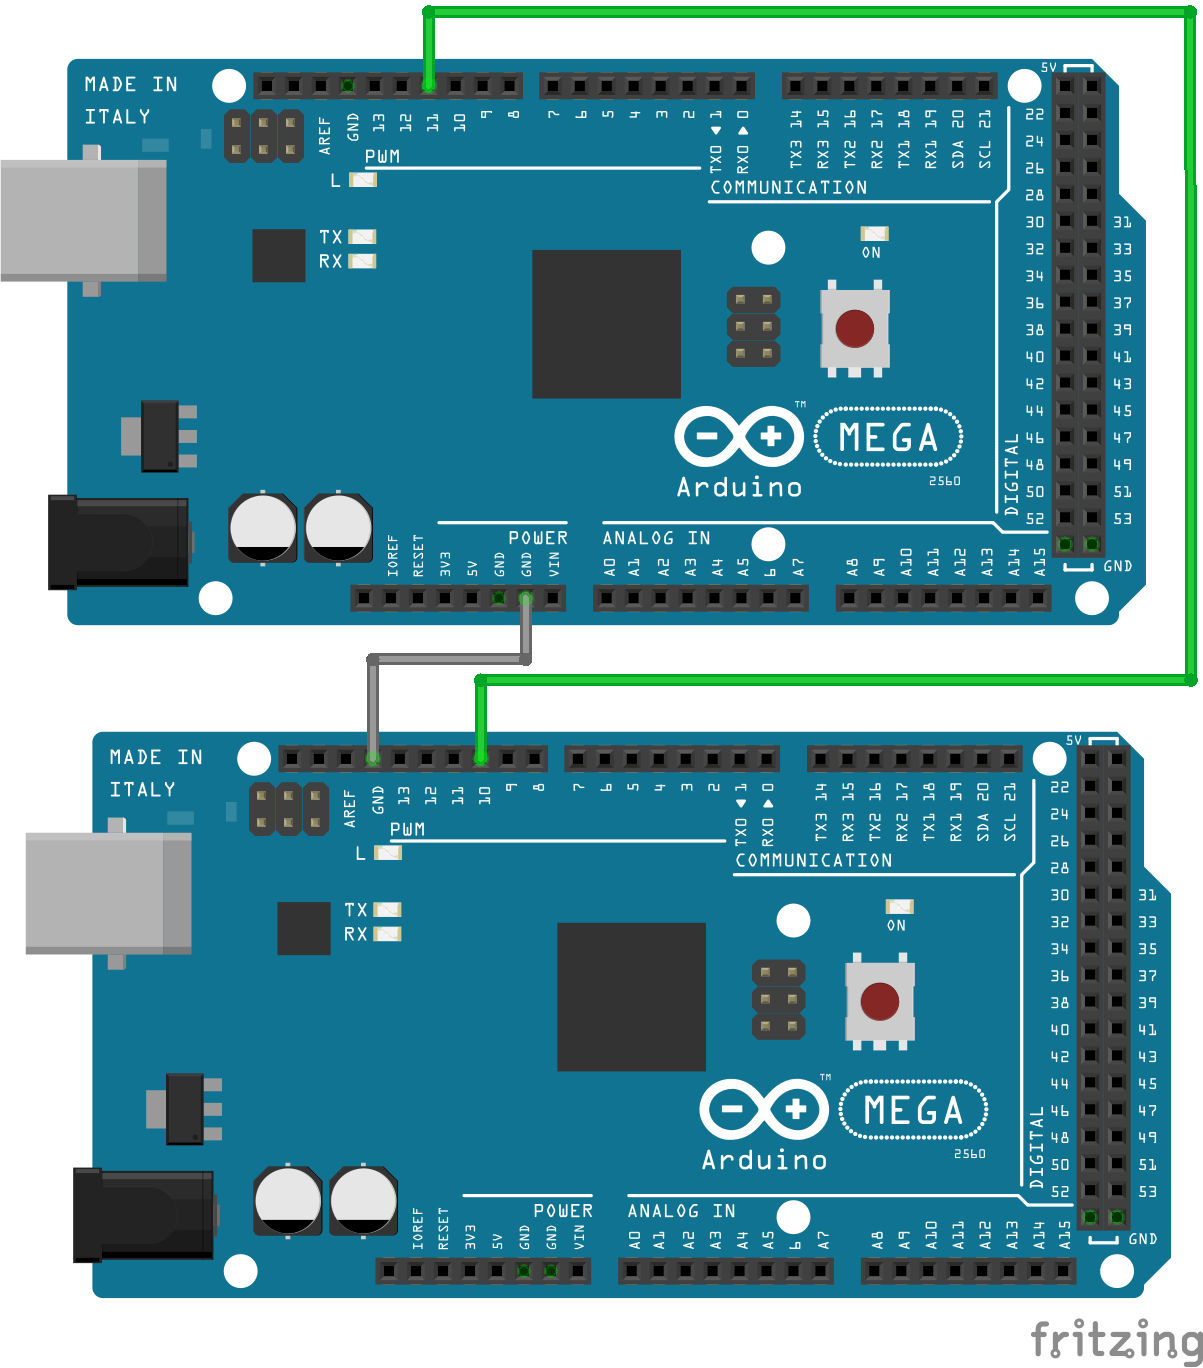
\includegraphics[width=10cm]{schematics/arduino-serial-communication-1}
  \caption{Connection of two Arduino Mega 2560 boards through UART in simplex
    (one-directional) data transfer mode.  The upper Arduino is the transmitter,
    the lower Arduino is the receiver.}
  \label{fig:arduino-serial-communication-1}
\end{figure}

The program code is the same for the both Arduino, the switch to the receiver
mode is done by connecting digital port 4 to the ground; if this port is not
connected, then the Arduino works in the transmitter mode. The full code is
shown in the listing \ref{listing:communication-serial-two-arduino-example}.

It should be noted that instead of a wire connecting RX-TX of two Arduino boards
we can use more sophisticated way of communication: a laser.  If we connect a
laser module (akin to the one that is shown on fig.
\ref{fig:arduino-laser-module}) to the TX of the first Arduino and point the
laser beam to a photoresistor connected to the RX pin of the second Arduino,
then we can transmit the data over the laser beam.  In this case we can clearly
see how the serial data transfer works: when we transmit the logical one, the
laser shines, when we transmit the logical zero that laser switches off.

One interesting ``side effect'' of data transfer over the laser beam is that the
power supply of the receiver and the transmitter are decoupled, thus they can
use different voltage values for logical levels.

\begin{figure}[ht]
  \centering
  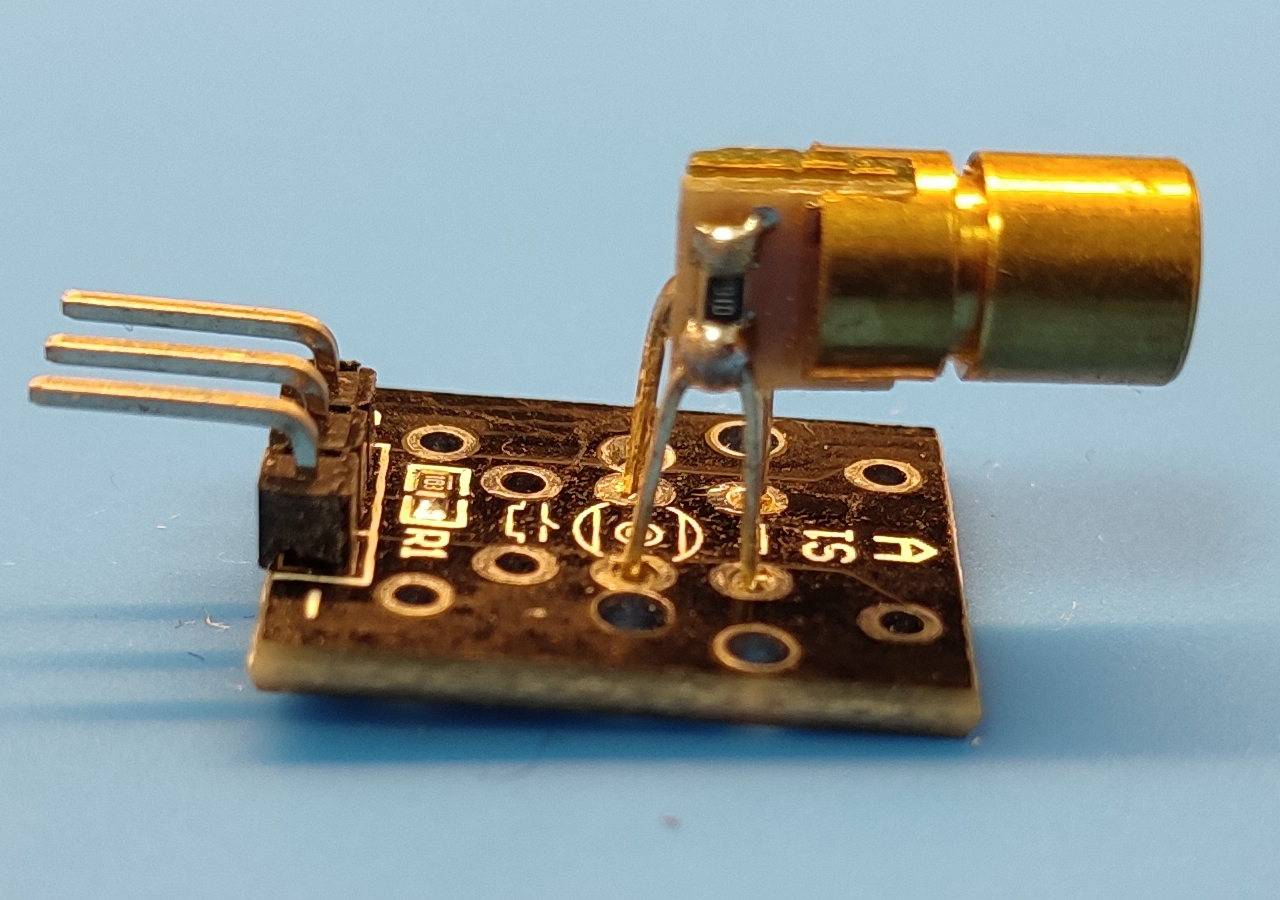
\includegraphics[width=8cm]{arduino-laser-module}
  \caption{A laser module for Arduino.}
  \label{fig:arduino-laser-module}
\end{figure}

\begin{figure}[ht]
  \centering
  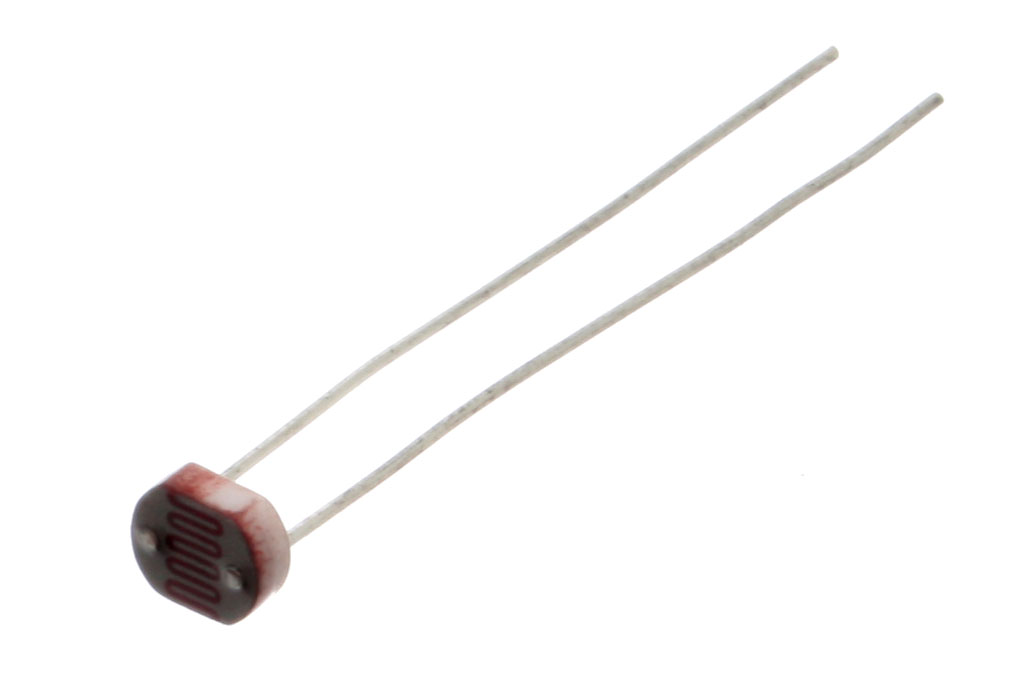
\includegraphics[width=8cm]{photoresistor}
  \caption{Photoresistor.}
  \label{fig:photoresistor}
\end{figure}

\begin{figure}[H]
  \centering
  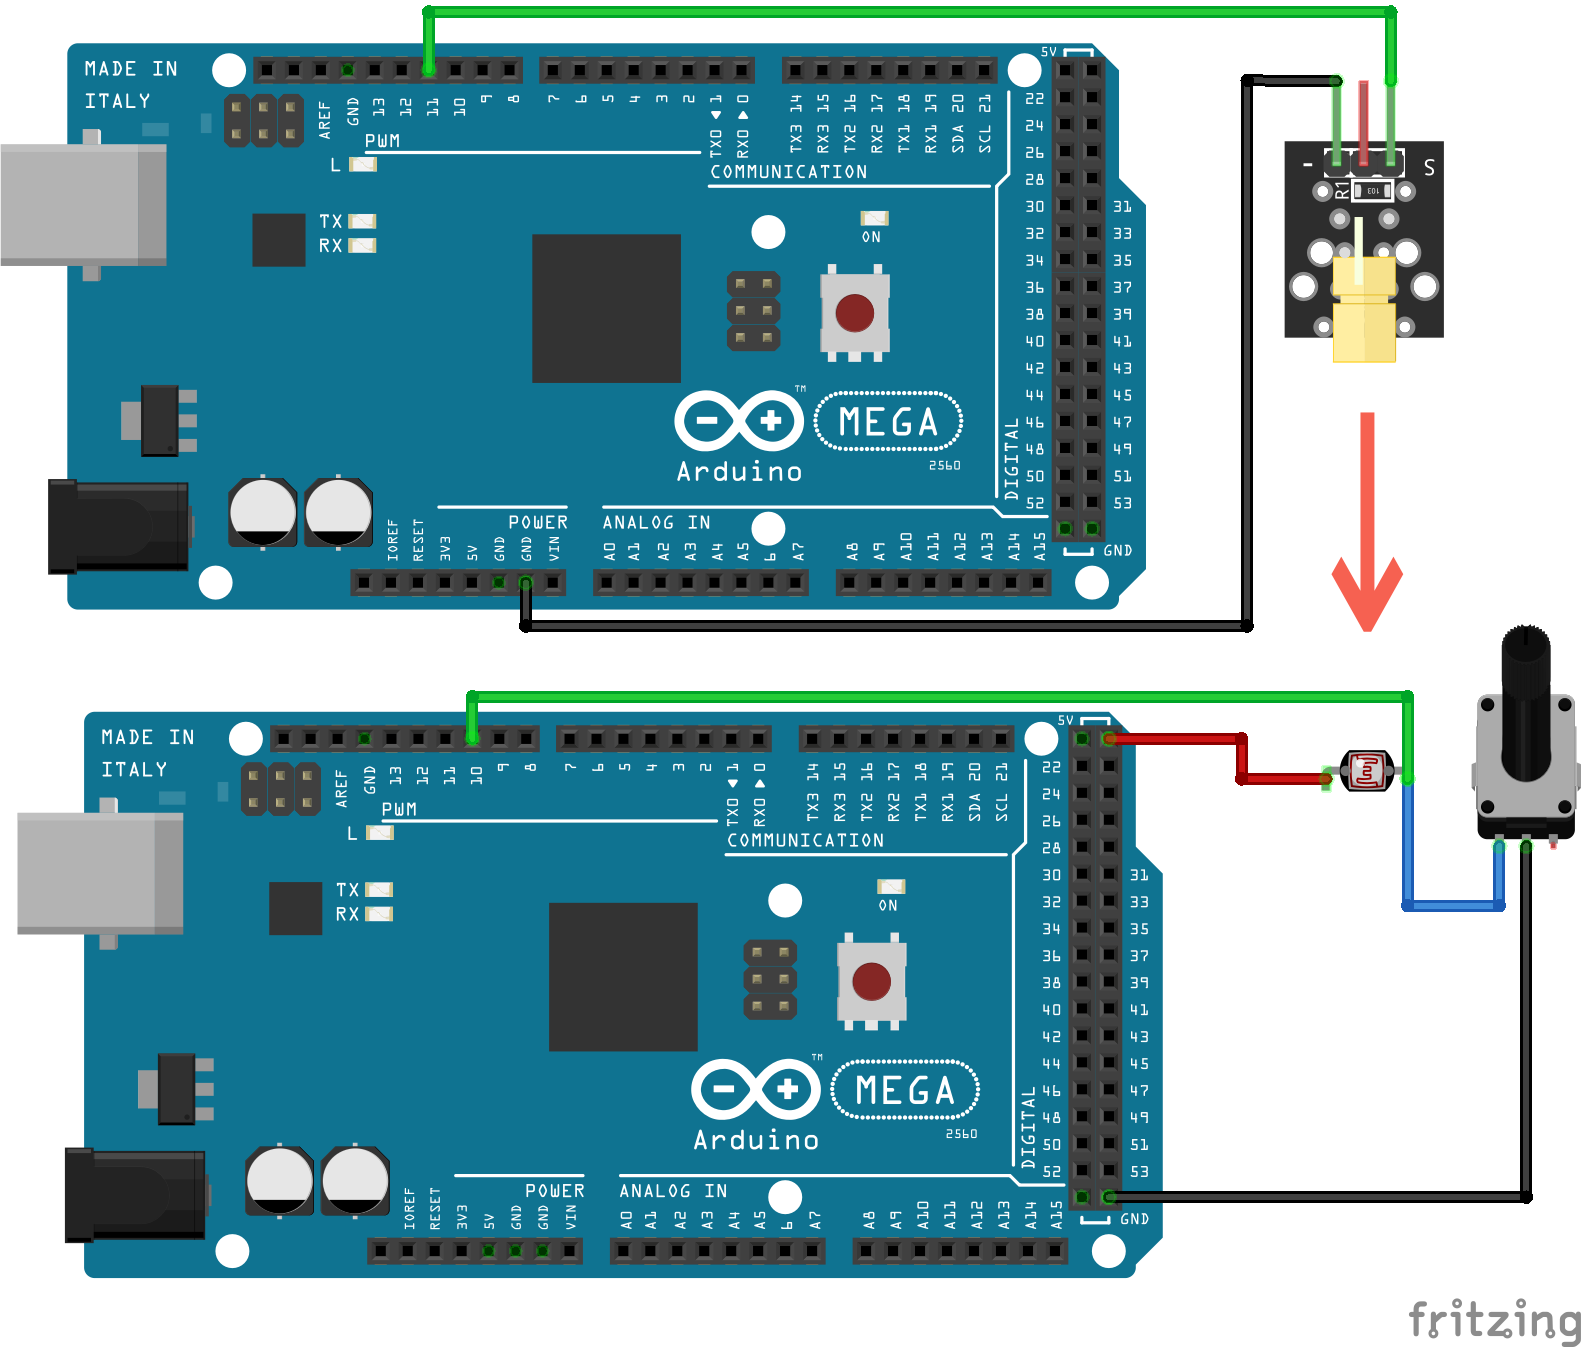
\includegraphics[width=10cm]{schematics/arduino-serial-communication-2}
  \caption{Connection of two Arduino Mega 2560 boards through UART using the
    laser beam as the data transfer medium.}
  \label{fig:arduino-serial-communication-2}
\end{figure}

The biggest problem when laser is used for such data transfer is to adjust the
light-sensitive sensor (a photoresistor) so an Arduino can distinguish ones from
zeroes.  The easiest way to do this is to use a voltage divider circuit where
$R_1$ is the photoresistor and $R_2$ is a potentiometer.  It will allow us to
adjust relation of $R_1$ to $R_2$ to change the voltage level that the Arduino
will receive when $R_1$ change.  By manual adjusting of the $R_2$ potentiometer
we can achieve the balance where the photoresistor $R_1$ will give us the
voltage level that is represents logical zero when it is not illuminated with
the laser; and when the laser beam illuminates the photoresistor, the
photoresistor will give us voltage level of logical one (see the
fig. \ref{fig:arduino-serial-communication-2}.)

\begin{listing}[H]
  \begin{minted}{cpp}
    #include <SoftwareSerial.h>
    const byte RX_PIN = 10;
    const byte TX_PIN = 11;
    SoftwareSerial software_serial(RX_PIN, TX_PIN);

    const byte SWITCH_PIN = 4;
    const byte LED_PIN = 13;

    void setup() {
      pinMode(SWITCH_PIN, INPUT_PULLUP);
      pinMode(LED_PIN, OUTPUT);
      Serial.begin(9600);
      software_serial.begin(600);
    }

    void transmit() {
      software_serial.print(1);
      delay(1000);
      software_serial.print(0);
      delay(1000);
    }

    void receive() {
      if (software_serial.available() > 0) {
        byte value = software_serial.read();
        Serial.print("VALUE: ");
        Serial.println(value);
        if (value == '1') {
          digitalWrite(LED_PIN, HIGH);
          Serial.println("ON");
          delay(1000);
        } else if (value == '0') {
          digitalWrite(LED_PIN, LOW);
          Serial.println("OFF");
          delay(1000);
        }
      }
    }

    void loop() {
      if (digitalRead(SWITCH_PIN) == HIGH) {
        transmit();
      } else {
        receive();
      }
    }
  \end{minted}
  \label{listing:communication-serial-two-arduino-example}
  \caption{An example of simplex (one-directional) connection of two Arduino
    boards through the serial port.}
\end{listing}


\end{document}
